%%%%%%%%%%%%%%%%%%%%%%%%%%%%%%%%%%%%%%%%%%%%%%%%%%%%%%%%%%%%%%%%%%%%%
% LaTeX Template: Project Titlepage Modified (v 0.1) by rcx
%
% Original Source: http://www.howtotex.com
% Date: February 2014
% 
% This is a title page template which be used for articles & reports.
% 
% This is the modified version of the original Latex template from
% aforementioned website.
% 
%%%%%%%%%%%%%%%%%%%%%%%%%%%%%%%%%%%%%%%%%%%%%%%%%%%%%%%%%%%%%%%%%%%%%%

\documentclass[12pt,letterpaper]{article}
\usepackage{fullpage}
\usepackage[top=2cm, bottom=4.5cm, left=2.5cm, right=2.5cm]{geometry}
\usepackage{amsmath,amsthm,amsfonts,amssymb,amscd,float}
\usepackage{lastpage}
\usepackage{enumerate}
\usepackage{fancyhdr}
\usepackage{mathrsfs}
\usepackage{xcolor}
\usepackage{graphicx}
\usepackage{listings}
\usepackage{hyperref}

\lstdefinestyle{Python}{
    language        = Python,
    frame           = lines, 
    basicstyle      = \footnotesize,
    keywordstyle    = \color{blue},
    stringstyle     = \color{green},
    commentstyle    = \color{red}\ttfamily
}


\newcommand{\HRule}[1]{\rule{\linewidth}{#1}}
\setcounter{tocdepth}{5}
\setcounter{secnumdepth}{5}



%-------------------------------------------------------------------------------
% HEADER & FOOTER
%-------------------------------------------------------------------------------
%\pagestyle{fancy}
%\fancyhf{}
%\setlength\headheight{15pt}
%\fancyhead[L]{Student ID: 1034511}
%\fancyhead[R]{Anglia Ruskin University}
%\fancyfoot[R]{Page \thepage\ of \pageref{LastPage}}
%-------------------------------------------------------------------------------
% TITLE PAGE
%-------------------------------------------------------------------------------

\begin{document}
{\fontfamily{cmr}\selectfont
\title{ \normalsize \textsc{}
		\\ [2.0cm]
		\HRule{0.5pt} \\
		\LARGE \textbf{\uppercase{FACE RECOGNITION}
		\HRule{2pt} \\ [0.5cm]
		\normalsize \today \vspace*{5\baselineskip}}
		}

\date{}

\author{
		Archit Kashyap(IMT2016064) \\
		Sonal Garg(IMT2016079)\\
		Vaibhav Kansagara(IMT2016068)
		}
\maketitle
\newpage
\tableofcontents
\newpage

%-------------------------------------------------------------------------------

\section{Pre-Processing}
At first we removed the images from the data-set where the pose was too much away from frontal.\\
For doing the pre-processing we first figure out the centre of the two eyes using eye-detectors and then we align such that two eye centres are parallel to the x-axis of the image(so that the image looks frontal even if the face is tilted to some extent) and resize the faces so that distance between the two eyes is 128 pixels and the image size is $256\times 256$. We don't keep the whole image but just the face which is recognised by the detector.\\ \\
First we define the align and resize function which takes in the eye centre co-ordinates and results out the output image which is aligned, cropped and resized.

\begin{lstlisting}[style=Python]
    def align_eye(self, image, leftEyeCenter, rightEyeCenter):
		dY = rightEyeCenter[1] - leftEyeCenter[1]
		dX = rightEyeCenter[0] - leftEyeCenter[0]
		angle = np.degrees(np.arctan2(dY, dX)) - 180
		desiredRightEyeX = 1.0 - self.desiredLeftEye[0]

		dist = np.sqrt((dX ** 2) + (dY ** 2))
		desiredDist = (desiredRightEyeX - self.desiredLeftEye[0])
		desiredDist *= self.desiredFaceWidth
		scale = desiredDist / dist

		eyesCenter = ((leftEyeCenter[0] + rightEyeCenter[0]) // 2, \
		(leftEyeCenter[1] + rightEyeCenter[1]) // 2)

		M = cv2.getRotationMatrix2D(eyesCenter, angle, scale)

		tX = self.desiredFaceWidth * 0.5
		tY = self.desiredFaceHeight * self.desiredLeftEye[1]
		M[0, 2] += (tX - eyesCenter[0])
		M[1, 2] += (tY - eyesCenter[1])

		(w, h) = (self.desiredFaceWidth, self.desiredFaceHeight)
		output = cv2.warpAffine(image, M, (w, h), flags=cv2.INTER_CUBIC)
		return output
\end{lstlisting}

Here given the desired distance between the two eyes and the image we find out the transformation matrix which rotates and resizes the image so that the distance between the two eyes is 128 pixels. It rotates the image in such a way that the two eyes are in parallel to x-axis of the image.
\newpage
For figuring out the location of left and right eye we use two different methods:
\begin{itemize}
    \item \textbf{HARR face and eye detectors}\\
    Here we use HARR cascade classifier to figure out the the face in the image and then crop out the face. We then use the eye classifier to figure out the eye from the cropped image.
    
    \begin{lstlisting}[style=Python]
    face_cascade = cv2.CascadeClassifier('./haarcascades/haarcascade_\
frontalface_default.xml')
    eye_cascade = cv2.CascadeClassifier('./haarcascades/haarcascade_eye.xml')
    for i in range(self.n):
	img = self.data[i]
	img_gray = gray[i]
			
	try:
	    faces = face_cascade.detectMultiScale(img_gray, 1.3, 5)
	    (x,y,w,h) = faces[0]
	    roi_gray = img_gray[y:y+h, x:x+w]
		roi_color = img[y:y+h, x:x+w]
				
		eyes = eye_cascade.detectMultiScale(roi_gray, 1.1, 3)
		(ex1,ey1,ew1,eh1) = eyes[0]
		(ex2,ey2,ew2,eh2) = eyes[1]
				
		if(ex1 < ex2):
		    lt_mid = [(ex1+(int)(ew1/2)), (ey1+(int)(eh1/2))]
		    rt_mid = [(ex2+(int)(ew2/2)), (ey2+(int)(eh2/2))]
		else:
		    rt_mid = [(ex1+(int)(ew1/2)), (ey1+(int)(eh1/2))]
		    lt_mid = [(ex2+(int)(ew2/2)), (ey2+(int)(eh2/2))]
	except:
		print("    "+str(i+1)+" failed")
		continue
	print("    "+str(i+1))
	res.append(fa.align_eye(roi_color, rt_mid, lt_mid))
    \end{lstlisting}
    Here in some images the classifier is not able to figure out the eyes or the face for that we have used try and except. In this for about 65\% images it works fine and for others out of 20 images only 8-13 images can be figured out, for images folder names "Suraj" the classifier couldn't figure out even a single image.
    
    \item \textbf{Dlib face detector}
    We tried using dlib's face detectors which detects out the face, eyes, noes, etc. from the face image.
    \begin{lstlisting}[style=Python]
    detector = dlib.get_frontal_face_detector()
    predictor = dlib.shape_predictor("shape_predictor_68_face_landmarks.dat")
    \end{lstlisting}
    We use the above predictor to figure out the eyes centre and then gave that to our align\_eye function defined above which gives out the aligned and cropped output image. Applying this worked for almost 80\% of all the images. But, again for images in folder named "Suraj" it couldn't figure out even a single image. We even tried just figuring out the face out of the image using Harr face classifier but didn't worked for "Suraj".
\end{itemize}
We save the pre-processed image to use them to train our model. \\
Some result from the above pre-processing:

\begin{figure}[!h]
    \centering
    
\includegraphics[width=0.3\linewidth]{image.jpg}
    \caption{Image}
    \label{fig1}
\end{figure}


\begin{figure}[!htb]
    \minipage{0.32\textwidth}
      
\includegraphics[width=\linewidth]{Harr.png}
      \caption{Harr(only face)}\label{fig2}
    \endminipage\hfill
    \minipage{0.32\textwidth}
      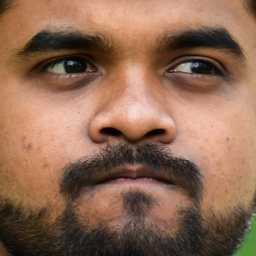
\includegraphics[width=\linewidth]{Harr_eye.png}
      \caption{Harr(face and eye)}\label{fig3}
    \endminipage\hfill
    \minipage{0.32\textwidth}%
      
\includegraphics[width=\linewidth]{dlib.png}
      \caption{dlib}\label{fig4}
    \endminipage
\end{figure}

We can clearly see that the face in Figure \ref{fig1} is slightly tilted, this can also be seen when we pre-process by using Harr detectors with only face detectors which just crop out the face from the image(Figure \ref{fig2}). After that when we use Harr with eye detectors or dlib which also detect eye centre and then realign the images we can see the face does not looks tilted (Figure \ref{fig3} and Figure \ref{fig4})

\section{Face Recognition}
\subsection{Train-test split}
After the pre-processing is done we move on to split the data-set into train and test such that ratio of data points in train and test for each class(person) is same, so that we better train our model and test it on all the classes. For doing this we load the saved pre-processed images each class at a time then applying train\_test\_split and appending them to the test and train data.

\subsection{Training the Model}
Now that we have pre-processed the image and split the data-set into train and test we use the training data to train out model. We use three different Models to train on the images.

\subsubsection{PCA(Opencv)}
For implementing PCA we have used cv2's implementation of Eigen faces:
    \begin{lstlisting}[style=Python]
    face_recognizer = cv2.face.EigenFaceRecognizer_create()
    face_recognizer.setNumComponents(50)
    face_recognizer.train(x_train, np.array(y_train))
    \end{lstlisting}
Here, we can set the number of eigen faces to use in the model. We will further look how the accuracy depends on this value.

\subsubsection{PCA(our implementation)}
We implemented our own PCA. The main theory behind PCA is that it tries to find out the Eigen faces which then helps us to reconstruct the image. For that we first have to find out the Eigen values and the corresponding eigen vectors of the matrix which denotes all the images in the dataset, but it is computationally hard that's we try to find the eigen values of $AA^T$ whose size is small thus making it feasible to compute. We then sort out the eigen values to get the top most eigen faces which will help us re-create the faces. After that we figure the eigen vectors from the matrix denoting the data and the eigen values. Then we generate the feature vector which we will use to train the models. To generate the feature vector related to each image we find the corresponding co-ordinate in the eigen plane for that image. After that we can train a ML model on the features to do face recognition. After that we use SVM as the ML model to do the face recognition.\\ \\
Below is the code to find out the eigen-vecotrs and eigen-values:
\newpage
    \begin{lstlisting}[style=Python]
    def fit(self, X):
        # here X -> [ --img1-- ]      
        #           [ --img2-- ]          
        #           [ --imgi-- ]       
    
        [total_images, image_sz] = X.shape
        
        self.mean = X.mean(axis = 0)
        X = X-self.mean

        if total_images > image_sz :
            cov = np.dot(X.T, X)
            [self.eigenvalues, self.eigenvectors] = np.linalg.eigh(cov)
        else:
            cov = np.dot(X, X.T)
            [self.eigenvalues, self.eigenvectors] = np.linalg.eigh(cov)
            self.eigenvectors = np.dot(X.T, self.eigenvectors)

            for i in range(total_images):
                self.eigenvectors[:,i] = self.eigenvectors[:,i]/np.linalg.norm(self.eigenvectors[:,i])
            

        #sort eigenvalues in descending order
        idx = np.argsort(-self.eigenvalues)
        self.eigenvalues = self.eigenvalues[idx]
        self.eigenvectors = self.eigenvectors[:,idx]
        
        # select only n_components
        self.eigenvalues = self.eigenvalues[0 : self.n_components].copy()
        self.eigenvectors = self.eigenvectors[ :, 0 : self.n_components].copy()
\end{lstlisting}
And the code to find the co-ordinates in the eigen plane corresponding to a specific image:
    \begin{lstlisting}[style=Python]
    def transform(self, X):
        # here X-> [--img--] dim=(no_of_images * image_size)
        if self.mean is None:
            return np.dot(X, self.eigenvectors)

        return np.dot(X - self.mean, self.eigenvectors)
    \end{lstlisting}

\subsubsection{LDA}
For implementing LDA we have used cv2's implementation of Fisher faces:
    \begin{lstlisting}[style=Python]
    face_recognizer = cv2.face.FisherFaceRecognizer_create()
    face_recognizer.train(x_train, np.array(y_train))
    \end{lstlisting}
    
\subsubsection{LBP}
For implementing LBP we have used cv2's implementation of LBPH faces:
    \begin{lstlisting}[style=Python]
    face_recognizer = cv2.face.LBPHFaceRecognizer_create()
    face_recognizer.train(x_train, np.array(y_train))
    \end{lstlisting}

\subsection{Testing the Models}
For getting the accuracy of the models we define a function which takes input as trained model, test data and rank(till which rank to check from the prediction output).
    \begin{lstlisting}[style=Python]
    def get_accuracy(face_recognizer, x_test, y_test, rank):
	y_pred_cnt = 0

	for i in range(len(x_test)):
		img = x_test[i]
		res = cv2.face.StandardCollector_create()
		face_recognizer.predict_collect(img, res)
		res = res.getResults(sorted=True)
		# tmp = min(range,len(res))
		for j in range(rank):
			(x,y) = res[j]
			if x==y_test[i]:
				y_pred_cnt += 1
				break
	return (y_pred_cnt/len(y_test))
    \end{lstlisting}

Now that we have trained the model and defined the function to calculate the accuracy given the model and rank.

\subsubsection{Rank 1 accuracy}

\begin{table}[!ht]
\begin{tabular}{lllll}
    & harr\_eye & dlib &  &  \\
PCA(opencv) & 0.53      & 0.79 &  &  \\
PCA(our) & 0.27    & 0.77 &  &  \\
LDA & 0.40      & 0.71 &  &  \\
LBP & 0.76      & 0.91 &  & 
\end{tabular}
\end{table}
Here harr\_eye stand for pre-processed input from harr face any eye classifier, while dlib tells that the pre-processed image comes from dlib.

\newpage
\subsubsection{Rank 3 accuracy}

\begin{table}[!ht]
\begin{tabular}{lllll}
    & harr\_eye & dlib &  &  \\
PCA(opencv) & 0.65      & 0.86 &  &  \\
PCA(our) & 0.41    & 0.91 &  &  \\
LDA & 0.48      & 0.78 &  &  \\
LBP & 0.77      & 0.96 &  & 
\end{tabular}
\end{table}

\subsubsection{Rank 10 accuracy}

\begin{table}[!ht]
\begin{tabular}{lllll}
    & harr\_eye & dlib &  &  \\
PCA(opencv) & 0.78      & 0.94 &  &  \\
PCA(our) & 0.59    & 0.98 &  &  \\
LDA & 0.62      & 0.84 &  &  \\
LBP & 0.84      & 0.98 &  & 
\end{tabular}
\end{table}

\subsubsection{Number of Eigenfaces vs accuracy}
Here we look at the accuracy values dependency on number of eigen faces used in case of PCA.

\begin{table}[!ht]
\begin{tabular}{lll}
\# Eigen faces & accuracy(PCA opencv) & accuracy(PCA our) \\
90             & 0.78     & 0.77\\
80             & 0.78     & 0.77\\
70             & 0.77     & 0.77\\
60             & 0.79     & 0.76\\
50             & 0.79     & 0.77\\
40             & 0.79     & 0.75\\
30             & 0.78     & 0.73\\
20             & 0.72     & 0.72\\
10             & 0.64     & 0.63\\
5              & 0.47     & 0.44
\end{tabular}
\end{table}

\subsection{Conclusion}
\begin{itemize}
    \item We can clearly see that in all cases we get the best accuracy with LBP followed by PCA and then LDA.
    \item Accuracy values increases as we increase the rank for all the models.
    \item Accuracy is relatively low for all models if we train them using the images which are pre-processed by Harr detectors than which are processed by dlib.
    \item When we train model using images pre-processed by Harr then the accuracy there a huge increase in accuracy values from Rank 3 to Rank 10.
    \item In case of PCA we see that as we increase the number of eigen faces the accuracy values increases and reaches the maximum around 50 eigen faces(for both opencv and out implementation) and then they start decreasing or becomes constant.
    \item Our implementation of PCA works better or almost as same opencv implementation on the images pre-processed by dlib. But our implementation of PCA doesn't works fine on the images pre-processed by Harr detectores.
\end{itemize}



\section{Open-face}
We used open face to get the 128 dimensional feature vector for the faces in the data-set. After that we use this feature vector and train our model, we used SVM for this.\\
We got an accuracy of 0.90 which is a good accuracy considering PCA and LDA.

\section{Gender}
For recognising gender from the given image we didn't change any code or used any other algorithm, rather we just trained all our existing models on a different data-set which contained only two classes: one of males and other of females. We gave all the males a single label and all the females another and then applied all the previous models.\\

\subsection{Rank 1 accuracy}

\begin{table}[!ht]
\begin{tabular}{ll}
model       & accuracy \\
PCA(opencv) & 0.90     \\
LDA         & 0.91     \\
LBP         & 0.99    
\end{tabular}
\end{table}

\newpage
\subsection{Rank 3 accuracy}

\begin{table}[!ht]
\begin{tabular}{ll}
model       & accuracy \\
PCA(opencv) & 0.95     \\
LDA         & 0.91     \\
LBP         & 1.0    
\end{tabular}
\end{table}

\subsection{Rank 10 accuracy}

\begin{table}[!ht]
\begin{tabular}{ll}
model       & accuracy \\
PCA(opencv) & 1.0     \\
LDA         & 0.92     \\
LBP         & 1.0    
\end{tabular}
\end{table}

 We got an accuracy of 0.93 using open face.We can clearly see that the accuracy of the models for gender recognition is very good.\\

%-------------------------------------------------------------------------------
% REFERENCES
%-------------------------------------------------------------------------------
\newpage
\section{References}
\url{https://www.pyimagesearch.com/2017/05/22/face-alignment-with-opencv-and-python/} \\
\url{http://reports-archive.adm.cs.cmu.edu/anon/anon/2016/CMU-CS-16-118.pdf} \\
\url{https://cmusatyalab.github.io/openface/}
}
\end{document}

